% !TEX root = ../main.tex

\section{Introduction and Paper Summary}

Retention time (RT) prediction is a core problem in LC-MS analysis because RT provides information that is complementary to MS/MS spectra. In the target paper, Kang et al.\ proposed \textbf{DeepGCN-RT}, a deep graph neural network for small-molecule RT prediction, and argued that previous RT-GNN models were still relatively shallow. Their main claim is that a \textbf{16-layer} graph convolutional architecture can be trained effectively once \textbf{residual connections}, \textbf{edge-aware message passing}, and an \textbf{attention/GRU readout} are introduced \cite{kang2023deepgcnrt}.

The paper reports three main contributions. First, on the SMRT benchmark, DeepGCN-RT improves the previously reported state of the art and reaches a test MAE of \textbf{26.55 s} and a MAPE of \textbf{0.033} (3.3\%). Second, after transfer learning from SMRT, the model improves performance on seven external chromatographic datasets with different conditions.

Our project focuses on an \textbf{independent PyTorch Geometric reimplementation} of the paper's core model and training pipeline. We used the authors' official repository only to clarify underspecified choices such as the readout structure, output normalization, and the exact transfer-learning hyperparameters. The final code in this repository was written independently and integrated into a clean training pipeline centered on PyG datasets, PyG data loaders, and our own \path{Networks/DeepGCNRT.py}. The final experiments reported here focus on SMRT base-model training and direct SMRT-initialized transfer learning on each MiniDataset under a \textbf{single shuffled train/validation/test split}.

\section{Model Architecture Reimplementation}

\subsection{Graph Construction}

Each molecule is converted from a canonical SMILES string into a graph
\(
G = (V, E)
\),
where atoms are nodes and bonds are directed edges. The preprocessing and featurization code in this repository produces node features of dimension \textbf{164} and edge features of dimension \textbf{11}. This closely follows the feature design described in the paper and the earlier GCN work by Kensert et al. \cite{kensert2021}, which the paper explicitly adopts \cite{kang2023deepgcnrt}.

The node representation contains 20 groups of atom-level features, including element type, degree, formal charge, hybridization, aromaticity, hydrogen-bond donor/acceptor flags, ring membership, chirality-related features, and several RDKit-derived physicochemical contributions. Edge features contain 5 groups of bond-level attributes, including bond type, stereo information, conjugation, ring membership, and rotatability.

\subsection{Message Passing Layer}

The reimplemented model follows the paper's notation as closely as possible. Let
\(
\mathbf{h}^{(l)}_u \in \mathbb{R}^d
\)
denote the hidden representation of source node \(u\) at layer \(l\), and let
\(
\mathbf{h}^{(l)}_{e_{uv}} \in \mathbb{R}^d
\)
denote the encoded edge feature between \(u\) and \(v\). The edge-aware message is

\begin{equation}
    \mathbf{m}^{(l)}_{uv} = \mathbf{h}^{(l)}_u + \mathbf{h}^{(l)}_{e_{uv}} .
\end{equation}

Following the best-performing setting used by the authors' released code, our implementation uses the \texttt{no\_relu} aggregation variant, so the attention weight is computed directly from the message:

\begin{equation}
    \alpha^{(l)}_{uv} =
    \frac{\exp \left( \mathbf{m}^{(l)}_{uv} \right)}
    {\sum\limits_{u' \in \mathcal{N}(v)} \exp \left( \mathbf{m}^{(l)}_{u'v} \right)} .
\end{equation}

Messages are aggregated at the destination node by weighted summation:

\begin{equation}
    \mathbf{m}^{(l)}_v =
    \sum\limits_{u \in \mathcal{N}(v)}
    \alpha^{(l)}_{uv} \odot \mathbf{m}^{(l)}_{uv} .
\end{equation}

The node state is then updated by a linear layer, ReLU, dropout, and residual connection:

\begin{equation}
    \mathbf{h}^{(l+1)}_v =
    \mathrm{Norm}
    \left(
    \mathrm{Dropout}
    \left(
        \mathrm{ReLU}
        \left(
            W^{(l)} \mathbf{m}^{(l)}_v
            \right)
        \right)
    \;+\;
    \mathbf{h}^{(l)}_v
    \right).
\end{equation}

In our final configuration, \(\mathrm{Norm}\) is the identity map, which matches the released DeepGCN-RT implementation for the edge-aware residual model.

\subsection{Readout and Prediction Head}

After \(L=16\) graph convolution layers, molecule-level embeddings are produced by an attentive readout with two refinement steps. The initial graph state is the sum of node embeddings:

\begin{equation}
    \mathbf{g}^{(0)} = \sum_{v \in V} \mathbf{h}^{(L)}_v .
\end{equation}

At each readout step, a graph-attention module propagates information from nodes to the graph state, and a GRU cell updates the graph embedding \cite{xiong2019}:

\begin{equation}
    \mathbf{c}^{(k)} = \mathrm{GAT}\!\left(\{\mathbf{h}^{(L)}_v\}, \mathbf{g}^{(k-1)}\right),
    \qquad
    \mathbf{g}^{(k)} = \mathrm{GRU}\!\left(\mathbf{c}^{(k)}, \mathbf{g}^{(k-1)}\right).
\end{equation}

The final molecular representation is passed through a two-layer MLP:
\[
    \mathbb{R}^{200} \rightarrow \mathbb{R}^{1024} \rightarrow \mathbb{R}^{1},
\]
with a ReLU between the two linear layers. The scalar output is the predicted RT in seconds.

\begin{algorithm}[t]
    \caption{Forward Pass of Our DeepGCN-RT Reimplementation}
    \begin{algorithmic}[1]
        \State Encode atom features with a linear layer: \(\mathbf{x}_v \mapsto \mathbf{h}^{(0)}_v\)
        \State Encode bond features with a linear layer: \(\mathbf{e}_{uv} \mapsto \mathbf{h}^{(0)}_{e_{uv}}\)
        \For{\(l = 0, \dots, 15\)}
        \State Compute edge-aware messages \(\mathbf{m}^{(l)}_{uv}\)
        \State Aggregate incoming messages with softmax-normalized weights
        \State Apply linear layer, ReLU, dropout, and residual connection
        \EndFor
        \State Initialize graph embedding by sum pooling over all nodes
        \For{\(k = 1, 2\)}
        \State Update graph embedding with graph attention and a GRU cell
        \EndFor
        \State Predict RT with the MLP head
    \end{algorithmic}
\end{algorithm}

\subsection{Assumptions and Design Decisions}

Several details are not fully specified in the paper text, so we made the following explicit choices:

\begin{enumerate}
    \item \textbf{Independent framework choice.} The authors' code is written with DGL. We reimplemented the same layer structure in \textbf{PyTorch Geometric} \cite{fey2019}, using \texttt{GATConv}, \texttt{global\_add\_pool}, and \texttt{GRUCell}. This changes the backend library and some internal operator details, even when the high-level computation graph is kept close to the paper.
    \item \textbf{Output normalization.} The released DeepGCN-RT code uses \texttt{output\_norm="none"} for the edge-aware attentive model. We follow that setting.
    \item \textbf{Aggregation update function.} The released code exposes three options: \path{relu_eps_beta}, \path{relu}, and \path{no_relu}. We adopt \path{no_relu}, because it is the default path used by the published training scripts for DeepGCN-RT.
    \item \textbf{Readout approximation.} The official DGL implementation directly uses \texttt{AttentiveFPReadout} \cite{xiong2019}. PyG does not provide a drop-in equivalent with the same implementation details, so we approximate the readout with graph attention plus \texttt{GRUCell} refinement. This is functionally close, but not guaranteed to be numerically identical.
    \item \textbf{Readout initialization.} The paper states that the initial graph embedding is obtained by summing node embeddings before the GRU refinement. Our readout reproduces exactly that behavior.
    \item \textbf{Loss implementation.} The paper reports Huber loss. In PyTorch, \texttt{SmoothL1Loss} is the standard Huber-style implementation, so we use it as the training objective.
\end{enumerate}

\section{Implementation Details}

The codebase was reorganized around three layers:

\begin{enumerate}
    \item \textbf{Dataset modules.} \path{Datasets/SMRT.py} and \path{Datasets/MiniDatasets.py} expose the shared interface used by the final reported experiments for preparing raw data, building PyG graphs, and loading train/validation/test splits.
    \item \textbf{Model definition.} \path{Networks/DeepGCNRT.py} contains the atom encoder, bond encoder, 16 residual edge-aware GCN layers, attentive readout, and final prediction head.
    \item \textbf{Training utilities.} \path{Train/lib/train_graph.py} implements the epoch loop, early stopping, scheduler stepping, checkpoint selection by validation loss, and metric logging.
\end{enumerate}

The implementation keeps the paper's layer widths and high-level structure unchanged: hidden dimension \(d=200\), 16 message-passing layers, two attentive readout steps, a 1024-unit dense hidden layer, dropout \(=0.1\), Adam optimizer, cosine warm restarts, and early stopping with patience 30.

One practical difference from the original repository is that our code unifies pretraining and transfer learning under the same training interface. This makes the pipeline easier to read and reuse. In the current version, the active code path uses a \textbf{single shuffled train/validation/test split} for transfer learning rather than the paper's repeated cross-validation loop on the transfer datasets.

\section{Experimental Setup}

\subsection{Datasets and Preprocessing}

We report only the datasets used in the final reproduction comparison. Table~\ref{tab:datasets} summarizes their sizes and the split sizes actually used by our current code.

\begin{table}[t]
    \centering
    \caption{Datasets used in the final reported experiments and the split sizes produced by our current loader (\(80\%/10\%/10\%\) after shuffling). All RT values are stored in seconds.}
    \label{tab:datasets}
    \resizebox{\textwidth}{!}{
        \begin{tabular}{lrrrrl}
            \toprule
            Dataset                  & Total  & Train  & Valid & Test  & Role in Report                    \\
            \midrule
            SMRT                     & 77,980 & 62,384 & 7,798 & 7,798 & Base pretraining dataset          \\
            Cao\_HILIC\_116          & 116    & 92     & 12    & 12    & Downstream MiniDataset evaluation \\
            Eawag\_XBridgeC18\_364   & 364    & 291    & 36    & 37    & Downstream MiniDataset evaluation \\
            FEM\_lipids\_72          & 72     & 57     & 7     & 8     & Downstream MiniDataset evaluation \\
            FEM\_long\_412           & 412    & 329    & 41    & 42    & Downstream MiniDataset evaluation \\
            FEM\_short\_73           & 73     & 58     & 7     & 8     & Downstream MiniDataset evaluation \\
            IPB\_Halle\_82           & 82     & 65     & 8     & 9     & Downstream MiniDataset evaluation \\
            LIFE\_new\_184           & 184    & 147    & 18    & 19    & Downstream MiniDataset evaluation \\
            LIFE\_old\_194           & 194    & 155    & 19    & 20    & Downstream MiniDataset evaluation \\
            MTBLS87\_147             & 147    & 117    & 15    & 15    & Downstream MiniDataset evaluation \\
            UniToyama\_Atlantis\_143 & 143    & 114    & 14    & 15    & Downstream MiniDataset evaluation \\
            \bottomrule
        \end{tabular}
    }
\end{table}

The preprocessing pipeline is identical across datasets:

\begin{enumerate}
    \item remove empty export columns such as \path{Unnamed:*};
    \item drop rows with missing RT or unparsable molecular structure;
    \item prefer SMILES, fall back to InChI when needed;
    \item canonicalize molecules with RDKit \cite{landrum2013};
    \item convert RT to seconds;
    \item transform molecules into PyG graphs and cache them to disk.
\end{enumerate}

One dataset-specific adjustment is important: in the MiniDatasets collection, the raw Excel files store RT in \textbf{minutes}, so our preprocessing multiplies those values by \(60.0\) before training. SMRT is already kept on the paper's second-based scale.

\subsection{Training Configuration}

Table~\ref{tab:training} lists the hyperparameters used in the code that generated the results currently stored in \path{Train/Results/DeepGCNRT/}.

\begin{table}[t]
    \centering
    \caption{Training settings used for the runs reported in this report. The MiniDataset stage uses direct SMRT-initialized transfer learning under a single shuffled split.}
    \label{tab:training}
    \resizebox{\textwidth}{!}{
        \begin{tabular}{llllll}
            \toprule
            Stage   & Target dataset(s) & Initialization        & Batch size & Epoch cap & Notes                                   \\
            \midrule
            Stage 1 & SMRT              & Random initialization & 64         & 200       & Base model training                     \\
            Stage 2 & Each MiniDataset  & Best SMRT checkpoint  & 8          & 200       & Direct transfer with one shuffled split \\
            \bottomrule
        \end{tabular}
    }
\end{table}

The following hyperparameters are shared across the reported stages unless otherwise noted: 16 GCN layers, hidden dimension 200, two attentive readout steps, prediction head \(200 \rightarrow 1024 \rightarrow 1\), dropout 0.1, Adam optimizer, \texttt{CosineAnnealingWarmRestarts} with \(T_0 = 200\), \texttt{SmoothL1Loss}, early stopping patience 30, and random seed 42.

\subsection{Deviations from the Original Experimental Protocol}

Reproduction reports are only useful when deviations are stated clearly. The most important differences between our current implementation and the paper are listed in Table~\ref{tab:deviations}.

\begin{table}[t]
    \centering
    \caption{Explicit deviations from the original paper and why they matter.}
    \label{tab:deviations}
    \resizebox{\textwidth}{!}{
        \begin{tabular}{p{3.2cm}p{5.1cm}p{5.1cm}p{4.1cm}}
            \toprule
            Aspect                        & Paper / official protocol                                                                                                                 & Our current implementation                                                                                                 & Expected impact                                                                                                         \\
            \midrule
            SMRT split                    & Fixed official split: 70,182 train and 7,798 test; train further split 9:1 for validation                                                 & \path{SMRT_train_set.txt} and \path{SMRT_test_set.txt} are merged, then reshuffled into 62,384/7,798/7,798                 & Makes SMRT results \emph{not strictly directly comparable} to the paper's reported test score                           \\
            Transfer evaluation           & 10 rounds of 10-fold cross-validation, averaged over seeds; batch size 8                                                                  & One shuffled train/validation/test split per MiniDataset; batch size 8                                                     & Simpler experimental flow, but no longer directly matches the paper's repeated-CV evaluation protocol                   \\
            Checkpoint selection          & Official transfer script evaluates the held-out fold every epoch and uses that same fold for early stopping and best-checkpoint selection & Our code selects the best checkpoint using a separate validation split and reports the test set only after model selection & Our protocol is methodologically cleaner, while the official protocol can produce optimistically biased transfer scores \\
            Effective training fraction   & Each transfer-learning fold trains on roughly 90\% of the dataset and does not reserve a separate validation split                        & Our transfer-learning runs train on 80\% of the dataset and reserve 10\% for validation                                    & On small datasets, the extra 10\% of training data in the official protocol can noticeably improve the reported score   \\
            Framework and readout backend & Official implementation uses DGL and its native \texttt{AttentiveFPReadout}                                                               & Our reimplementation uses PyG and approximates the readout with graph attention plus \texttt{GRUCell}                      & Backend-level operator differences can change numerical behavior even when the architecture is conceptually matched     \\
            Hyperparameter adaptation     & Official results are reported under the released transfer-learning workflow and repeated-CV setting                                       & We intentionally use one fixed hyperparameter set across all MiniDatasets and do not tune settings per dataset             & This makes the comparison cleaner, but it does not maximize performance on each individual transfer dataset             \\
            Transfer dataset scope        & Paper discusses 7 external RPLC datasets                                                                                                  & We also ran Cao\_HILIC\_116, FEM\_short\_73, and MTBLS87\_147 because they appear in the released codebase                 & Extra coverage, but those rows are supplementary rather than main-paper reproduction                                    \\
            Repetition strategy           & 3 runs on SMRT; 10\(\times\)10 CV on transfer learning                                                                                    & One run per stage in the final report                                                                                      & Easier to manage, but variance estimation is weaker than in the paper                                                   \\
            \bottomrule
        \end{tabular}
    }
\end{table}

\section{Results and Comparison}

\subsection{SMRT Benchmark}

Our reproduced SMRT base model reaches a test MAE of \textbf{26.65 s}, a MedAE of \textbf{12.53 s}, a MAPE of \textbf{0.0332}, and an \(R^2\) of \textbf{0.90}. Numerically, this is very close to the paper's reported DeepGCN-RT result of 26.55 s MAE \cite{kang2023deepgcnrt}. The comparison should still be interpreted with care because our current SMRT loader reshuffles the merged official train and test files before creating the final 80/10/10 split, so the held-out set is not identical to the paper's fixed benchmark split.

\begin{table}[t]
    \centering
    \caption{SMRT test-set performance. Baseline values are reproduced from Table 1 of the paper \cite{kang2023deepgcnrt}.}
    \label{tab:smrt-main}
    \begin{tabular}{lcccc}
        \toprule
        Method             & MAE (s) & MedAE (s) & MAPE  & \(R^2\) \\
        \midrule
        DeepGCN-RT (paper) & 26.55   & 12.38     & 0.033 & 0.89    \\
        DeepGCN-RT (ours)  & 26.65   & 12.53     & 0.033 & 0.90    \\
        GCN (paper)        & 29.40   & 15.02     & 0.040 & 0.89    \\
        DNNpwa (paper)     & 39.62   & 25.08     & 0.050 & 0.85    \\
        GNN-RT (paper)     & 39.87   & 25.24     & 0.050 & 0.85    \\
        \bottomrule
    \end{tabular}
\end{table}

This is the strongest part of the reproduction. Even with the split mismatch, the base model behaves as expected: the large SMRT dataset supports stable optimization, the 16-layer residual graph stack does not collapse, and the edge-aware attentive readout transfers well enough to serve as a reasonable source model for the later stages.

\begin{figure}[t]
    \centering
    \IfFileExists{Figures/smrt_base_scatter_report.png}{
        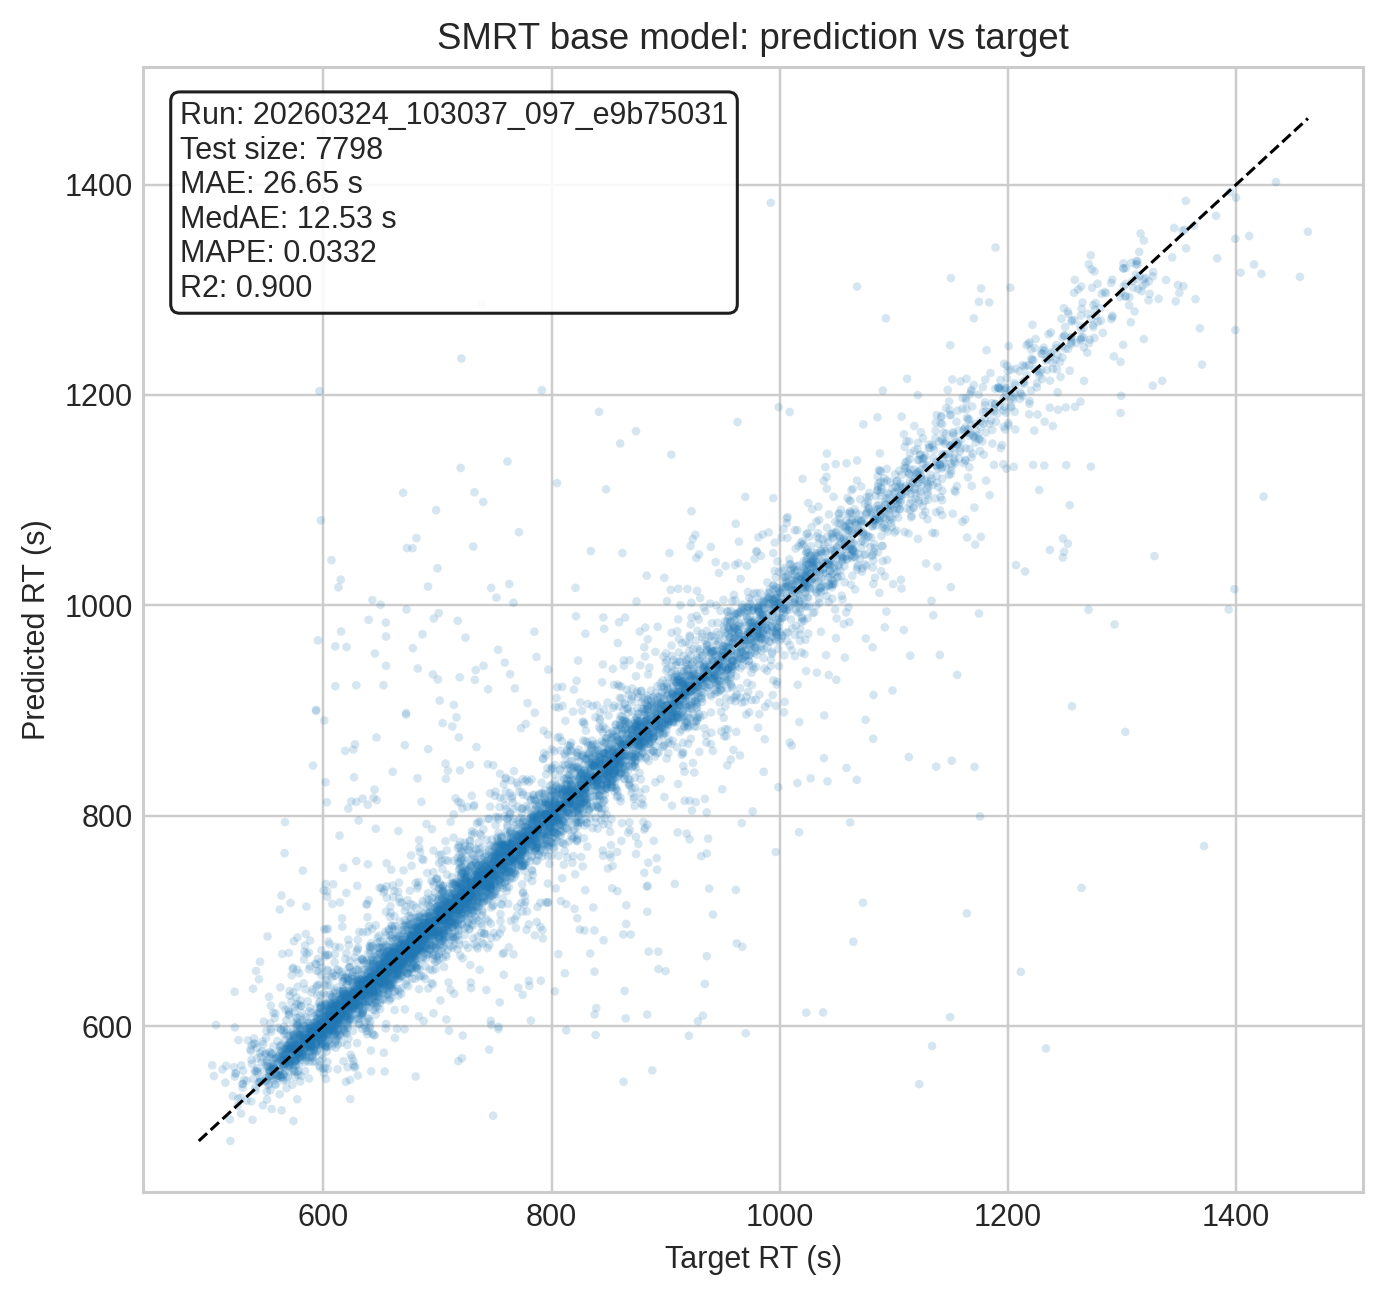
\includegraphics[width=0.72\textwidth]{Figures/smrt_base_scatter_report.png}
    }{}
    \caption{Prediction scatter of the reproduced SMRT base model on the held-out test split. The concentration of points around the diagonal reflects the near-paper-level MAE obtained by our implementation.}
    \label{fig:smrt-scatter}
\end{figure}

\begin{figure}[t]
    \centering
    \IfFileExists{Figures/smrt_mae_comparison_report.png}{
        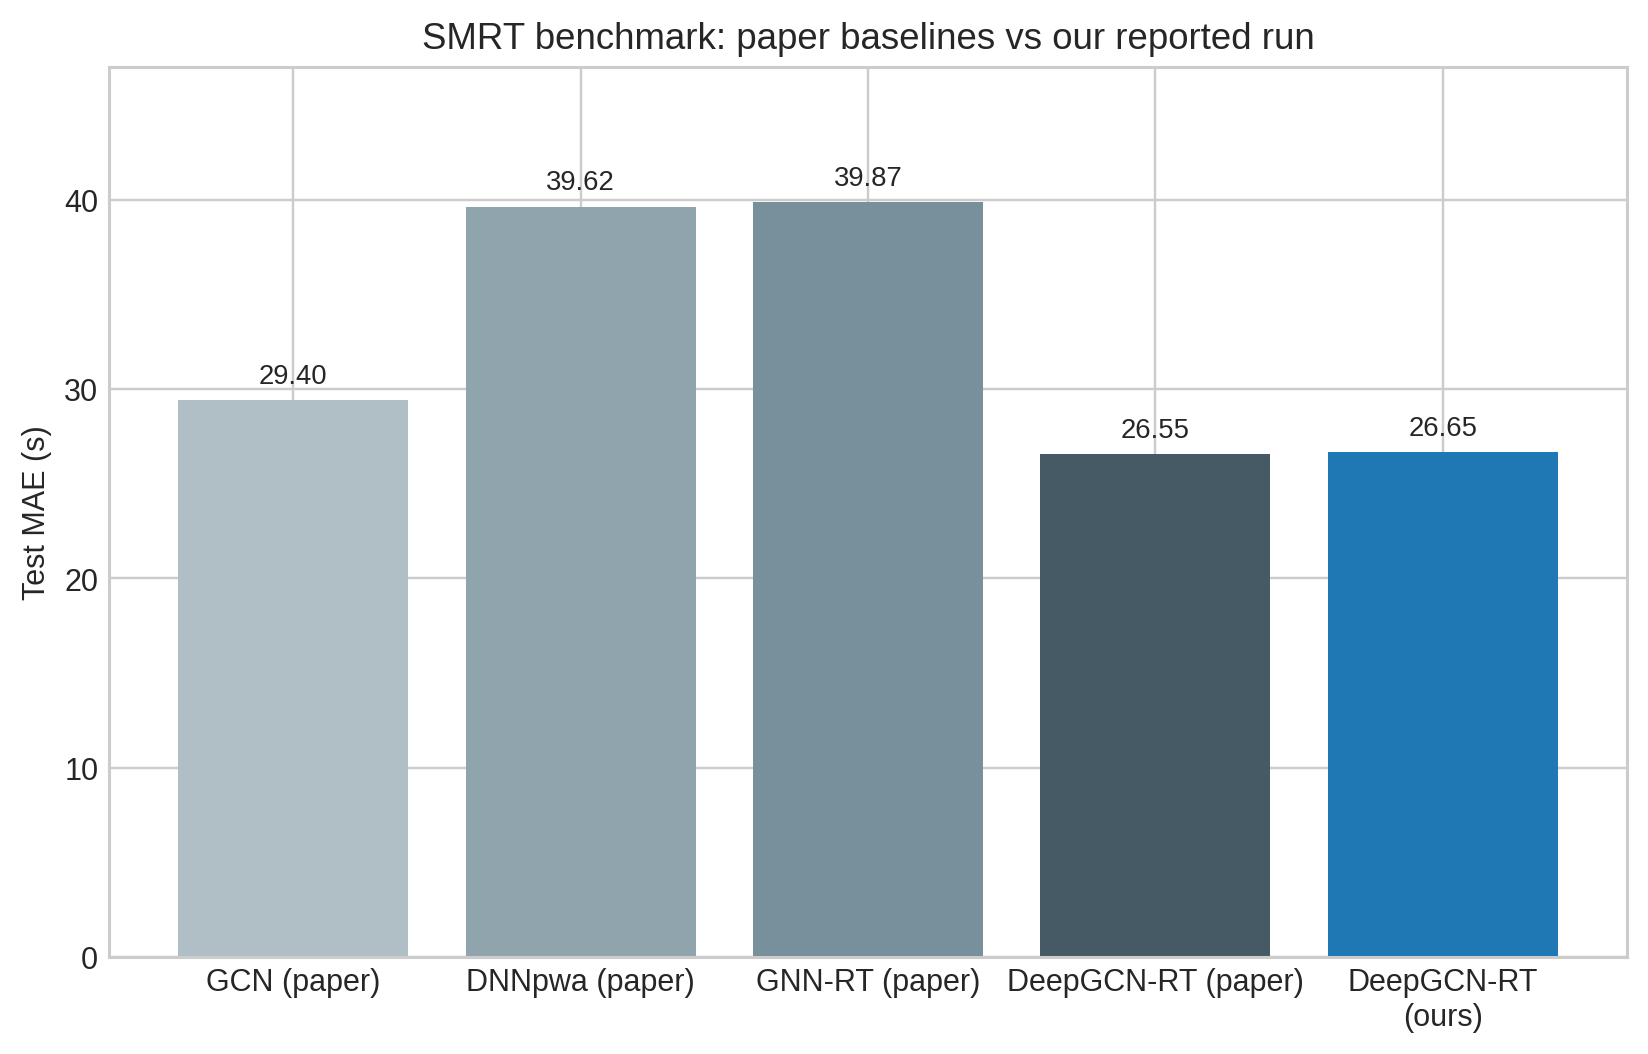
\includegraphics[width=0.74\textwidth]{Figures/smrt_mae_comparison_report.png}
    }{}
    \caption{SMRT benchmark MAE comparison between the paper's published baselines and our reproduced DeepGCN-RT run.}
    \label{fig:smrt-mae}
\end{figure}

\subsection{MiniDataset Transfer Learning on the Seven Paper Datasets}

Table~\ref{tab:transfer-seven} compares our single-split transfer-learning runs against the seven datasets explicitly discussed in the paper. In this group, \textbf{UniToyama\_Atlantis\_143} is the only dataset where our MAE is better than the official DeepGCN-RT number. \textbf{LIFE\_new\_184} and \textbf{LIFE\_old\_194} remain relatively close to the paper. The largest deterioration appears on \textbf{FEM\_long\_412}, where our MAE is worse by 92.38 s.

\begin{table}[t]
    \centering
    \caption{Transfer-learning MAE comparison on the seven datasets explicitly discussed in the paper. Official numbers are taken from Table 4 of the paper \cite{kang2023deepgcnrt}; our runs use a single shuffled train/validation/test split rather than repeated cross-validation.}
    \label{tab:transfer-seven}
    \begin{tabular}{lrrrr}
        \toprule
        Dataset                  & Official MAE (s) & Our MAE (s) & Notes         & Gap (s) \\
        \midrule
        Eawag\_XBridgeC18\_364   & 45.97            & 61.78       & test \(n=37\) & +15.81  \\
        FEM\_lipids\_72          & 74.48            & 96.81       & test \(n=8\)  & +22.33  \\
        FEM\_long\_412           & 110.89           & 203.27      & test \(n=42\) & +92.38  \\
        IPB\_Halle\_82           & 21.20            & 31.62       & test \(n=9\)  & +10.42  \\
        LIFE\_new\_184           & 18.13            & 21.16       & test \(n=19\) & +3.03   \\
        LIFE\_old\_194           & 12.07            & 16.14       & test \(n=20\) & +4.07   \\
        UniToyama\_Atlantis\_143 & 50.03            & 42.94       & test \(n=15\) & -7.09   \\
        \bottomrule
    \end{tabular}
\end{table}

Across the seven paper datasets, the official DeepGCN-RT MAEs average 47.54 s, whereas our single-split runs average 67.67 s, for a mean gap of +20.14 s. This difference is large enough that it cannot be explained by implementation error alone. The most important reason is the evaluation protocol: the released transfer-learning script performs 10-fold cross-validation but also monitors the held-out fold during training and uses that same fold for early stopping and checkpoint selection. Our pipeline instead uses a separate validation split and reports the test set only after model selection. That choice is more rigorous, but it usually produces less optimistic numbers.

\begin{figure}[t]
    \centering
    \IfFileExists{Figures/mini_all_mae_comparison.png}{
        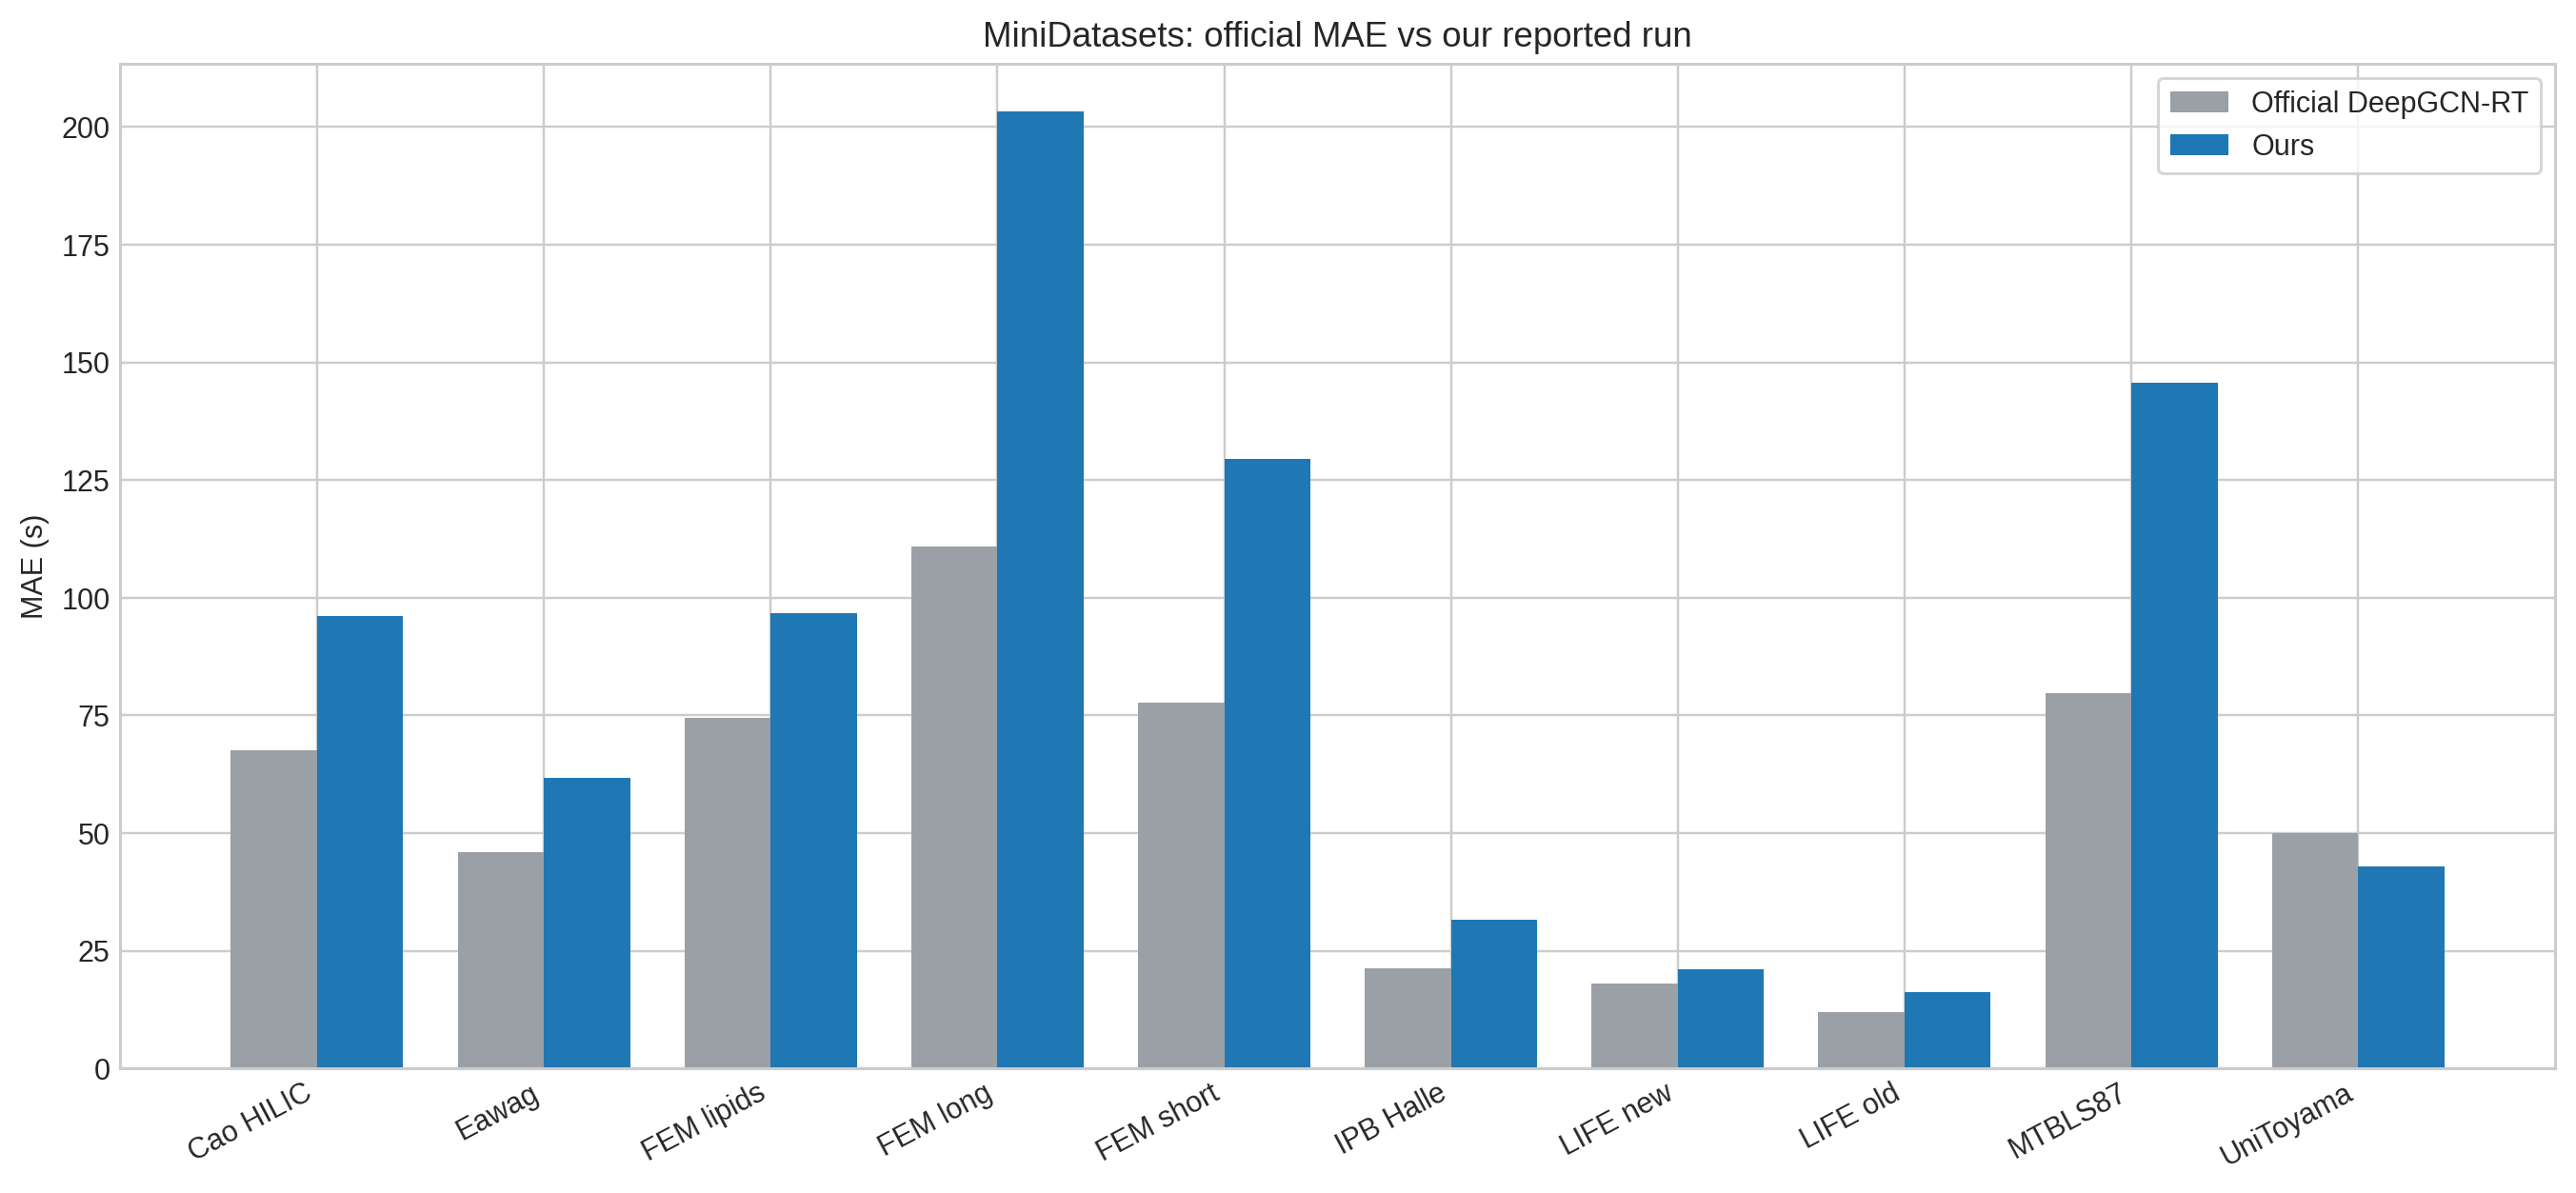
\includegraphics[width=\textwidth]{Figures/mini_all_mae_comparison.png}
    }{}
    \caption{MiniDataset MAE comparison between the official DeepGCN-RT results and our single-split transfer-learning runs.}
    \label{fig:mini-all-mae}
\end{figure}

\subsection{Additional Datasets Present in the Official Code}

The official repository also includes three additional datasets outside the main seven-dataset table. We ran those datasets as supplementary experiments under the same single-split protocol.

\begin{table}[t]
    \centering
    \caption{Supplementary comparison on extra datasets included in the released codebase.}
    \label{tab:transfer-extra}
    \begin{tabular}{lrrrr}
        \toprule
        Dataset         & Official MAE (s) & Our MAE (s) & Notes         & Gap (s) \\
        \midrule
        Cao\_HILIC\_116 & 67.64            & 96.21       & test \(n=12\) & +28.57  \\
        FEM\_short\_73  & 77.70            & 129.60      & test \(n=8\)  & +51.90  \\
        MTBLS87\_147    & 79.74            & 145.60      & test \(n=15\) & +65.86  \\
        \bottomrule
    \end{tabular}
\end{table}

These extra datasets reinforce the same pattern as the main table: performance is feasible, but highly unstable once the transfer problem becomes data-poor and the evaluation is reduced to a single split.

\begin{figure}[t]
    \centering
    \IfFileExists{Figures/mini_test_size_vs_gap.png}{
        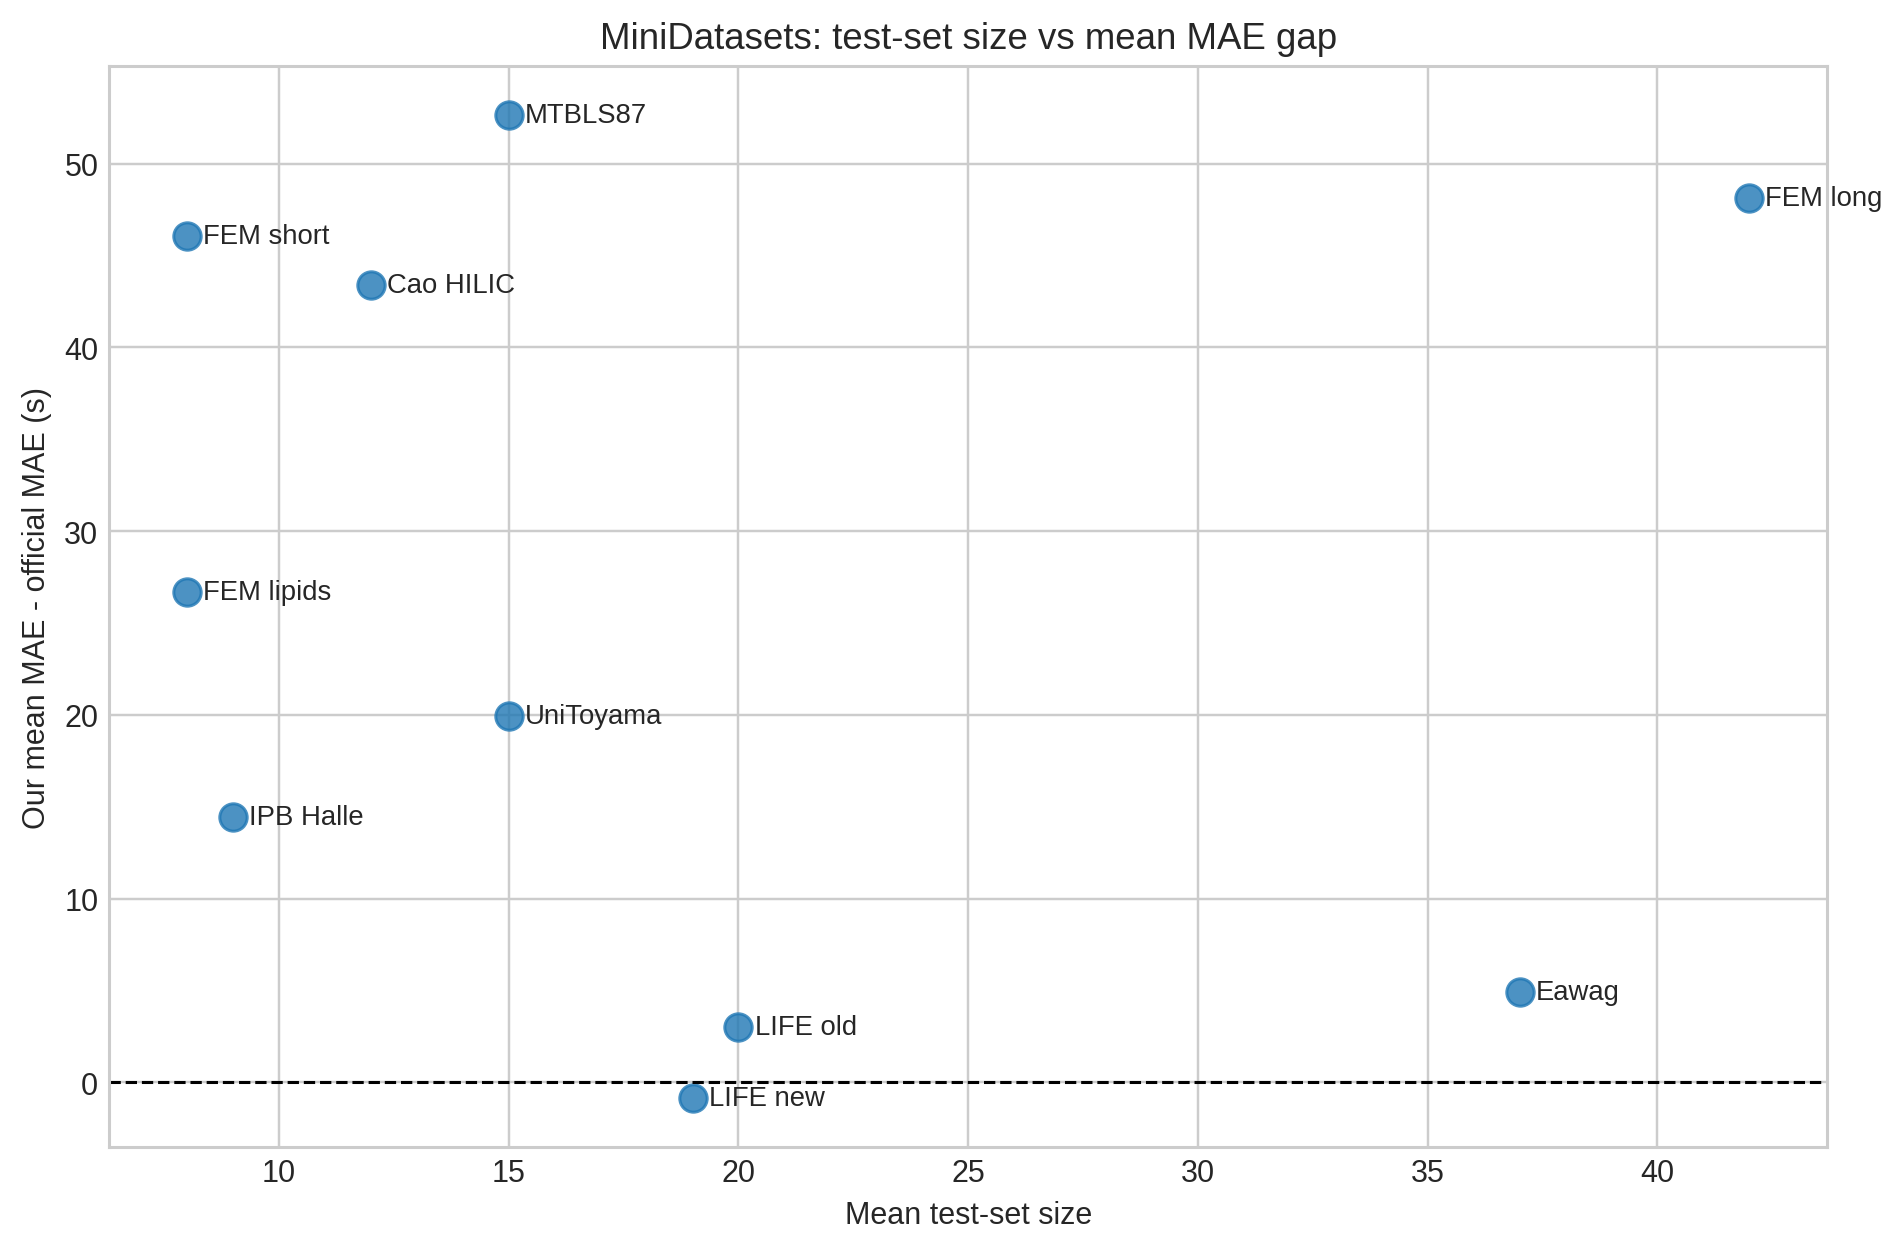
\includegraphics[width=0.78\textwidth]{Figures/mini_test_size_vs_gap.png}
    }{}
    \caption{MiniDataset test-set size versus MAE gap. The figure highlights how volatile the comparison becomes once the held-out split contains only 8 to 20 molecules.}
    \label{fig:mini-testsize-gap}
\end{figure}

\section{Analysis and Discussion}

\subsection{Why Do Some Results Match Well While Others Do Not?}

The easiest result to match is the SMRT base model. SMRT is large enough that the optimization dynamics are smooth, the best checkpoint is well defined, and the architecture can show its intended strength: depth plus residual connections without obvious over-smoothing. That is why our reimplementation gets close to the paper even though the split itself is not identical.

The downstream MiniDataset results are much harder to match. The paper reports repeated 10-fold cross-validation, whereas our runs use one shuffled train/validation/test split. More importantly, the released \path{transfer_learning.py} script evaluates the held-out fold every epoch and uses that same fold for checkpoint selection and early stopping. This means the official fold score is not a fully untouched test score. Our implementation deliberately avoids that practice and uses a dedicated validation split instead. Methodologically, our setting is cleaner; numerically, it is also more conservative.

The amount of training data also differs. In the official 10-fold setup, each fold trains on roughly 90\% of the molecules. In our 80/10/10 split, only 80\% of the data is used for fitting because 10\% is reserved for validation and 10\% for test. On datasets with only 72, 82, or 116 compounds, that 10\% reduction in training data is non-trivial. Combined with the stricter model-selection protocol, it is enough to explain why our MiniDataset scores are usually slightly worse than the paper's.

There is also a framework-level source of mismatch. The official model is implemented in DGL and uses its native \texttt{AttentiveFPReadout}. Our model is implemented in PyG, and the readout is approximated with \texttt{GATConv} and \texttt{GRUCell} because PyG does not provide a drop-in equivalent with the same internals. This is a reasonable reimplementation choice, but it is still an approximation. Backend-level numerical differences in message passing, batching, and readout can accumulate and cause small performance shifts even when the architecture is conceptually aligned.

\subsection{Sensitivity to Hyperparameters and Randomness}

The reported transfer-learning results are clearly sensitive to split composition and early stopping. The best epoch ranges from \textbf{3} on Cao\_HILIC\_116 to \textbf{89} on FEM\_long\_412, which already suggests that the smaller datasets do not provide a uniformly stable validation signal. When the test set contains only 8 to 12 compounds, one or two difficult molecules can noticeably change the final MAE.

Because we intentionally fixed the hyperparameters instead of tuning them per dataset, the current report does not claim that these are the best achievable MiniDataset numbers for our implementation. Rather, they are the outcomes of a clean, consistent transfer-learning protocol. A more aggressive optimization campaign could tune learning rate, weight decay, scheduler behavior, and early-stopping patience separately for each MiniDataset and might close part of the remaining gap.

\subsection{Strengths and Weaknesses of the Architecture}

The reimplementation still supports the paper's main architectural claims. First, a 16-layer graph model can be trained effectively for RT prediction when residual connections and a stable readout are present; our SMRT result is direct evidence of that. Second, the model transfers non-trivially across datasets: UniToyama plus the two LIFE datasets remain competitive even under a stricter single-split evaluation. Third, the architecture is expressive enough to preserve useful information from both atom and bond features, which is exactly where an edge-aware GNN should help relative to simpler baselines.

The weaknesses are mostly practical rather than conceptual. DeepGCN-RT is still data-hungry on small transfer sets, and its downstream quality depends strongly on evaluation protocol. A separate validation split is cleaner, but it further reduces the already limited training data. In addition, exact framework-level equivalence is difficult when the released implementation depends on DGL-specific components such as \texttt{AttentiveFPReadout}.

\subsection{What We Learned from the Reimplementation}

The reimplementation made two points especially clear. The first is that the model architecture itself is reproducible: once the missing details from the paper are fixed explicitly, a clean PyG implementation can recover near-paper performance on SMRT. The second is that experimental protocol matters almost as much as architecture. Choices about split generation, validation usage, checkpoint selection, and backend implementation can easily dominate the final comparison on small transfer datasets.

\section{Conclusion and Lessons Learned}

Our independent PyTorch Geometric reimplementation of DeepGCN-RT successfully reproduces the core model behavior. On the SMRT benchmark, the reproduced base model reaches \textbf{26.65 s} MAE, which is very close to the paper's published \textbf{26.55 s}.

The main reproduction gap appears on the MiniDatasets. Under our single shuffled split, the transfer-learning results are generally worse than the paper's repeated cross-validation results, with UniToyama as the main exception and LIFE\_new/LIFE\_old remaining comparatively close. The most defensible interpretation is therefore not that the architecture failed, but that the downstream evaluation is highly protocol-sensitive once the datasets become small. The official transfer-learning workflow uses the held-out fold during model selection and also keeps more molecules in the training portion of each fold, so its reported numbers are expected to look better than a stricter train/validation/test protocol.

The main lesson from this project is that reproducing a paper requires reproducing both the model and the measurement procedure. For DeepGCN-RT, the architectural reimplementation is not the difficult part; the harder issue is aligning data splits, checkpoint selection, readout implementation details, and downstream evaluation with enough fidelity that the final numbers can be compared fairly.


\section*{Use of Generative AI}

Generative AI tools (including Claude and ChatGPT) were used during this project as a supporting tool for understanding, organization, and communication. Specifically, AI assistance was used to help explain parts of the original codebase to grab some details, to help us learn the new PyG library much more easily, and improve the grammar of our report.

AI tools were not used as a substitute for running experiments or validating results. All code execution, experimental outputs, numerical results, interpretation of model performance, and final decisions were checked and approved by the project team. The reported results are based on our own implementation and experiments.

We acknowledge that AI-generated suggestions may contain inaccuracies. Therefore, all AI-assisted content was reviewed against the original paper, the official repository, and maed sure that the new expression aligns with what we want to express in the final report.

\begin{thebibliography}{9}

    \bibitem{kang2023deepgcnrt}
    Q. Kang, P. Fang, S. Zhang, H. Qiu, and Z. Lan,
    \newblock ``Deep graph convolutional network for small-molecule retention time prediction,''
    \newblock \emph{Journal of Chromatography A}, vol. 1711, 464439, 2023.

    \bibitem{deepgcnrtcode}
    Q. Kang et al.,
    \newblock ``DeepGCN-RT official source code and pretrained models,''
    \newblock GitHub repository: \url{https://github.com/kangqiyue/DeepGCN-RT}.

    \bibitem{kensert2021}
    A. Kensert, R. Bouwmeester, K. Efthymiadis, P. Van Broeck, G. Desmet, and D. Cabooter,
    \newblock ``Graph convolutional networks for improved prediction and interpretability of chromatographic retention data,''
    \newblock \emph{Analytical Chemistry}, vol. 93, pp. 15633--15641, 2021.

    \bibitem{xiong2019}
    Z. Xiong, D. Wang, X. Liu, F. Zhong, X. Wan, X. Li, Z. Li, X. Luo, K. Chen, H. Jiang, et al.,
    \newblock ``Pushing the boundaries of molecular representation for drug discovery with the graph attention mechanism,''
    \newblock \emph{Journal of Medicinal Chemistry}, vol. 63, pp. 8749--8760, 2019.

    \bibitem{fey2019}
    M. Fey and J. E. Lenssen,
    \newblock ``Fast graph representation learning with PyTorch Geometric,''
    \newblock \emph{arXiv preprint}, arXiv:1903.02428, 2019.

    \bibitem{landrum2013}
    G. Landrum,
    \newblock ``RDKit: A software suite for cheminformatics, computational chemistry, and predictive modeling,'' 2013.
    \newblock \url{https://www.rdkit.org}

\end{thebibliography}
